\section*{Aufgabe 4.1a)}
\begin{lstlisting}[caption=Output des Beispielaufrufs,label=lst:fouriertestoutput,language=]
Vektor eins: 
v1 =

   1
   2
   3
   4
\end{lstlisting}



\section*{Aufgabe 5.1}
Im Folgenden wurde mittels der Fourier-Analyse eine Möglichkeit der Bildkomprimierung
getestet. Das verwendete Bild ohne Veränderungen ist in \fref{orig} abgebildet.

\begin{figure}[htb]
\centering
  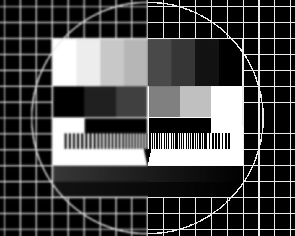
\includegraphics[width=0.7\textwidth,keepaspectratio]{../tmp/testbild}
  \caption{Orginales Bild ohne Komprimierung}
  \label{fig:orig}
\end{figure}

\section*{Aufgabe 5.1a)}

Zunächst wurde eine Funktion \lref{cut_rect} geschrieben, die den Rand des Graustufen-Bildes
schwärzt, die Pixel also auf 0 setzt. Die Breite wird hierbei in Abhängigkeit
des Kompressionsparameters $ρ \in [0,1]$ so eingestellt, dass $hb\cdot ρ^2$
nicht-triviale Pixel verbleiben, wobei $h$ die Höhe und $b$ die Breite des
Bildes in Pixeln ist.

\lstinputlisting[firstline=1,lastline=10,firstnumber=1,label=lst:cut_rect,caption={cut\_rect.m}]{../code/cut_rect.m}

Wird die Funktion aus \lref{cut_rect} unter Verwendung von $ρ^2 = 0.4$ auf das
Bild in \fref{orig} angewendet, so erhält man die in \fref{1a} gezeigte Abbildung.

\begin{figure}[htb]
\centering
  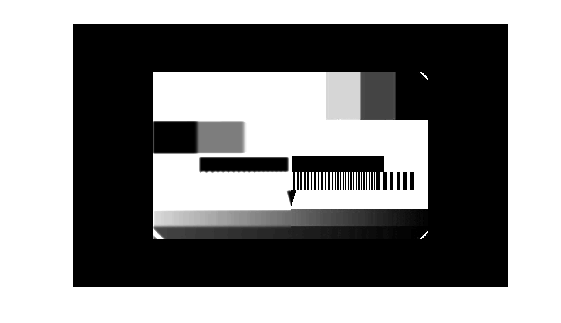
\includegraphics[width=0.7\textwidth,keepaspectratio]{../tmp/eins_a}
  \caption{Bild mit Rand bei $ρ^2 = 0.4$}
  \label{fig:1a}
\end{figure}

\section*{Aufgabe 5.1b)}
\section*{Aufgabe 5.1c)}
\section*{Aufgabe 5.1d)}
\section*{Aufgabe 5.1e)}